\documentclass[conference]{IEEEtran}
\IEEEoverridecommandlockouts
% The preceding line is only needed to identify funding in the first footnote. If that is unneeded, please comment it out.
\usepackage{cite}
\usepackage{amsmath,amssymb,amsfonts}
\usepackage{algorithmic}
\usepackage{graphicx}
\usepackage{textcomp}
\usepackage{xcolor}
\def\BibTeX{{\rm B\kern-.05em{\sc i\kern-.025em b}\kern-.08em
		T\kern-.1667em\lower.7ex\hbox{E}\kern-.125emX}}

\begin{document}
	
	\title{Report Title}
	
	\makeatletter
	\newcommand{\linebreakand}{%
	\end{@IEEEauthorhalign}
	\hfill\mbox{}\par
	\mbox{}\hfill\begin{@IEEEauthorhalign}
	}
	\makeatother
	
	\author{\IEEEauthorblockN{1\textsuperscript{st} SHALOMI FERNANDES}
		\IEEEauthorblockA{\textit{Faculty of Engineering } \\
			\textit
			Bristol, UK \\
			email address or ORCID}
		\and
		\IEEEauthorblockN{2\textsuperscript{nd} FANGNAN WEI}
		\IEEEauthorblockA{\textit{Faculty of Engineering } \\
			\textit
			Bristol, UK \\
			email address or ORCID}
		\linebreakand %
		\IEEEauthorblockN{3\textsuperscript{rd} JIADONG XU}
		\IEEEauthorblockA{\textit{Faculty of Engineering } \\
			\textit
			Bristol, UK \\
			email address or ORCID}
		\and
		\IEEEauthorblockN{4\textsuperscript{th} JIAHUI LIU}
		\IEEEauthorblockA{\textit{Faculty of Engineering } \\
			\textit
			Bristol, UK \\
			ye23356@bristol.ac.uk}
	}
	
	\maketitle
	
	\begin{abstract}
		This article utilizes machine learning techniques to predict the specificity of T cell receptors (TCRs), which play a key role in the immune system's response to pathogens and cancer cells. Our research focuses on the broad diversity of TCR sequences in the VDJdb dataset to understand their interactions with specific epitopes. We have developed a method that includes the preprocessing of TCR sequence data, we have used techniques such as Encoding, computational distance matrix, classification, dimensionality reduction, clustering techniques to process the VDJdb dataset, and we have also built an algorithm aimed at predicting antigen specificity. Our innovative computational approach is expected to overcome the limitations of current empirical approaches and significantly improve the effectiveness of immunotherapies and personalized medicine. This article presents the results of our research on the predictive accuracy of these methods and discusses potential improvements and future research directions.
	\end{abstract}
	
	\section{Introduction}
	This article aims to predict the specificity of T cell receptors (TCRs) by machine learning techniques. TCRs are a key component of the immune system, which is able to recognize and respond to antigens presented by pathogens or cancerous cells through a highly variable molecular structure. This diversity is primarily generated through the recombination of variable (V), diversity (D), and junction (J) gene fragments, allowing TCRs to bind to a variety of peptides presented by major histocompatibility complex (MHC) molecules. However, due to the complexity and high variability of peptide-MHC-TCR interactions, the use of sequence data to predict the specificity of TCRs remains a challenge. Most of the existing traditional methods rely on empirical data, which often cannot accurately capture the nuances of antigen recognition. Therefore, this research aims to develop an innovative computational method that can more accurately simulate and predict TCR behavior through in-depth analysis of the vast TCR sequence data in the VDJdb database, which is expected to drive the development of personalized medicine and immunotherapy.
	
	Predicting TCR specificity is critical for advancing immunotherapies and designing targeted therapies. The project involves preprocessing TCR sequence data, encoding, calculating distances, classification, clustering, dimensionality reduction techniques, and developing algorithms for predicting antigen specificity. We focus on extracting meaningful patterns from TCR sequences using dimensionality reduction and clustering techniques, with the aim of developing robust predictive models. Our approach aims not only to enhance the understanding of TCR-antigen interactions, but also to advance personalized medicine by facilitating the development of more effective immunotherapies.
	
	By combining computational methods with immunological insights, our research explores new areas of immunoinformatics, paving the way for breakthroughs in the understanding and therapeutic utilization of the immune system. This research has great potential to enhance the efficacy of personalized medicine and immunotherapy, and to address the limitations of current empirical approaches through innovative computational methods.
	
	\section{Literature Review}
	
	"GIANA allows computationally-efficient TCR clustering and multi-disease repertoire classification by isometric transformation" introduces a TCR alignment algorithm GIANA based on geometric isometric transformation, a new computational tool designed to improve the efficiency and accuracy of T cell receptors. GIANA not only improves calculation speed (600 times faster than TCRdist without sacrificing accuracy), but also facilitates fast queries of large reference queues. It successfully identified novel disease-associated TCRs and classified unseen samples in a variety of diseases, including cancer, infectious diseases, and autoimmune diseases.
	
	"TCR meta-clonotypes for biomarker discovery with tcrdist3 enabled identification of public, HLA-restricted clusters of SARS-CoV-2 TCRs" introduces a new framework to classify biochemically similar TCRs into "meta-clonotypes". Researchers used the newly developed open source software package tcrdist3 to analyze TCR data from COVID-19 patients to create and quantify meta-clonotypes, providing a more powerful tool for identifying disease-associated TCR patterns. Application of this method identified 1,831 public TCR metaclonotypes associated with SARS-CoV-2, and significant HLA restriction was observed. Meta-clonotypes were more frequently detected in the TCR repertoires of patients with specific HLA genotypes than exact amino acid matches.
	
	"T cell receptor sequence clustering and antigen specificity" describes clustering techniques for classifying TCR sequences based on their biological similarity and antigen specificity. Technological advances have made TCR sequencing data widely available, and there is increasing interest in understanding TCR-epitope interactions to predict disease outcome, track treatment efficacy, and stratify patients for treatment. This review discusses several sequencing-based methods, including sequence alignment, analysis of short TCR motifs, and the use of various computational tools to predict TCR binding based on structural and sequence data, highlighting the challenges of these methods, such as the need for large data set and the complexity of predicting protein interactions based on sequence data alone. The paper also explores future directions for improving TCR sequence analysis, showing that integrating more sophisticated machine learning models and structural data can improve the predictive accuracy of these methods.
	
	
	\section{Methodology}
	In this paper, the data are preprocessed, encoded, distance calculation, classified, clustered, dimensionally reduced, and predicted. The encoding method used in this article is one-hot, BLOSUM 62 and GIANA Encoding. The distance calculation method used in this article is TCRDist, GIANA and Levenshtein. The classification method used in this article is RandomForestClassifier, LogisticRegresion and SVM. The clustering methods used in this article is Agglomerative Hierarchical clustering and DBSCAN. The dimensionality methods used in this article is PCA, t-SNE and UMAP.
	
	
	\subsection{Pre-Processing}
	This article first preprocesses the dataset to preserve the available columns 'complex.id','gene', 'cdr3', 'v.segm', 'j.segm', 'species', 'mhc.a', 'mhc.b', 'mhc.class', 'antigen.epitope', 'vdjdb.score'. Remove the row where the missing value of 'v.segm', 'j.segm' is located, as well as the duplicate row. Delete the row with a value of 0 in the 'vdjdb.score' column. The processed dataset is used for encoding.
	
	\subsection{Encoding Methods}
	\subsubsection{One-Hot Encoding} \
	
	One-hot encoding\cite{b2} is a technique for representing categorical variables as binary vectors. In this encoding, the value of each variable is represented as a vector of length equal to the number of possible values, with only one element being 1 (representing the category to which the variable belongs) and all other elements being 0.
	
	Mathematical Description:
	
	Let \( X \) be a categorical variable with a finite set \( C \) of \( N \) categories, such that:
	\[ X \in C = \{ c_1, c_2, \ldots, c_N \} \]
	
	Here, each \( c_i \) represents a distinct category.
	
	Corresponding to each category \( c_i \) of \( X \), we define a one-hot vector \( d_i \) as a binary vector of length \( N \). This vector has all elements set to 0 except for the \( i \)-th element, which is set to 1.

	For a given category \( c_i \), its one-hot vector \( d_i \) is given by:
	\[ d_i = (0, 0, \ldots, 1, \ldots, 0) \]
	
	Here, the 1 is in the \( i \)-th position of the vector \( d_i \), indicating the presence of category \( c_i \).
	
	We can also define one-hot encoding using an indicator function \( I \) as follows:
	\[ d_{i}[j] = I(j = i) \]
	
	Where:
	\[ I(true) = 1 \quad \text{and} \quad I(false) = 0 \]
	
	The indicator function \( I \) returns 1 when its argument is true (when \( j = i \)), and 0 otherwise.
	
	The one-hot vector \( d_i \) can be represented as:
	\[ d_i = [d_{i}[1], d_{i}[2], \ldots, d_{i}[N]] \]
	
	Where:
	\[ d_{i}[j] = 
	\begin{cases} 
		1 & \text{if } j = i \\ 
		0 & \text{if } j \neq i 
	\end{cases}
	\]
	
	In this article, we define the one\_hot\_encode\_sequence function, which takes two parameters: the sequence to be encoded and a list of all possible amino acids. The function creates a two-dimensional array with the number of rows equal to the length of the sequence and the number of columns equal to the number of types of amino acids, iterates through each amino acid in the sequence, and sets the value of the corresponding position to 1 if the amino acid is in a given list of amino acids, indicating that the amino acid appears, otherwise it is 0. The one\_hot\_encode\_sequence function is called for each sequence in the 'cdr3' column, and the result is stored in a new column named cdr3\_one\_hot\_encoded.
	
	
	In the one\_hot\_encode file in the encoders folder, a function called one\_hot\_encode\_cdr3 is defined that accepts the CDR3 sequence and parameter max\_length to set the maximum length of the encoded sequence. Iterate through each amino acid in the CDR3 sequence, check if the amino acid is in the standard amino acid letter, and if the amino acid is in the standard letter, set the value of the corresponding position to 1, which implements one-hot encoding. Depending on the length of the sequence, the encoded array is truncated or filled to ensure that all encoded sequences have the same length.
	
	\subsubsection{BLOSUM 62 ENCODING} \
	
	BLOSUM 62\cite{b2} encoding is a protein sequence encoding method that is based on the score of the BLOSUM (Blocks Substitution Matrix) substitution matrix. The BLOSUM 62 substitution matrix is derived from statistical analysis of a large number of known protein sequences to assess the similarity between two amino acids. In the BLOSUM 62 encoding, each amino acid is mapped to a vector whose length is equal to the number of rows of the substitution matrix. Each element in the vector represents the similarity score of that amino acid to the corresponding row in the substitution matrix.
	
	In this paper, we import BLOSUM62 module from Biopython to define a function encode\_sequence\_with\_blosum62 (sequence, blosum62\_matrix) with protein sequences and BLOSUM62 matrices as inputs. For each amino acid in the input sequence, its corresponding BLOSUM62 code is retrieved from the matrix. If the amino acid is not found in the matrix, the zero vector is used as its code. Convert the encoded list of amino acids into a numpy array for further processing.
	
	\subsubsection{GIANA ENCODING} \
	
	GIANA Encoding\cite{b2} converts TCR sequences into numerical representations of fixed dimensions. The core idea of GIANA Encoding is to use Autoencoder to learn the low-dimensional representation of TCR sequences. The Autoencoder consists of an encoder and a decoder that can learn a compressed representation of the data. In GIANA Encoding, the encoder is responsible for mapping the TCR sequence to the low-dimensional space, while the decoder is responsible for mapping the low-dimensional representation back to the original TCR sequence space.
	
	This paper defines a function GIANA\_encoder that accepts a list of TCR sequences and an optional parameter ST with a default value of 3. The function first checks whether there are CDR3 sequences of alpha and beta strands in the TCR sequence, then extracts the CDR3 sequences of alpha and beta chains, and finally encodes the CDR3 sequences of alpha and beta chains. Finally, the encoding results of the alpha and beta chains are connected along the column direction to form an overall encoding result.
	
	
	This article defines another function GIANA\_encoder\_pd encode CDR3 sequences. First, the CDR3 sequences of the alpha and beta chains are obtained, and then the encoding results of the alpha and beta chains are concatenated and converted into Python lists.
	\subsection{Distance Calculation}
	
	\subsubsection{TCRDist} \
	
	TCRDist\cite{b2}\cite{b3} is a toolkit for calculating TCR distances, which can be calculated based on their sequence characteristics (e.g., CDR3 sequences) and possibly other information (e.g., expression patterns of TCRs).
	
	For a given set of TCR sequences, the distances between all possible pairs are calculated, and the results are formed into a distance matrix, each element in the matrix represents the distance or similarity between the pairs, and once the distance matrix is calculated, visualization tools can be used to show the similarity or difference between the TCRs.
	
	In this paper, we first define the main distance calculation function distance\_cal, obtain the parts of the TCR sequence (such as cdr3 alpha and beta chains, V and J segments, etc.) from the parameters, and then call different auxiliary functions to calculate the distance between the different parts. The \_distance\_cal function is an auxiliary function of the distance\_cal, which is used to calculate the distance between sequences, and the distance between sequences is calculated by dynamic programming. The distance\_categorical function is used to calculate the distance between categorical data (e.g., V and J segments, MHC, etc.), which simply compares whether two classifications are the same and gives the corresponding distance. dist\_to\_matrix function converts the calculated distance vector into a distance matrix. Fig.1. shows the result of TCR Distance Matrix Calculation.
	
	\begin{figure}[h]
		\centering
		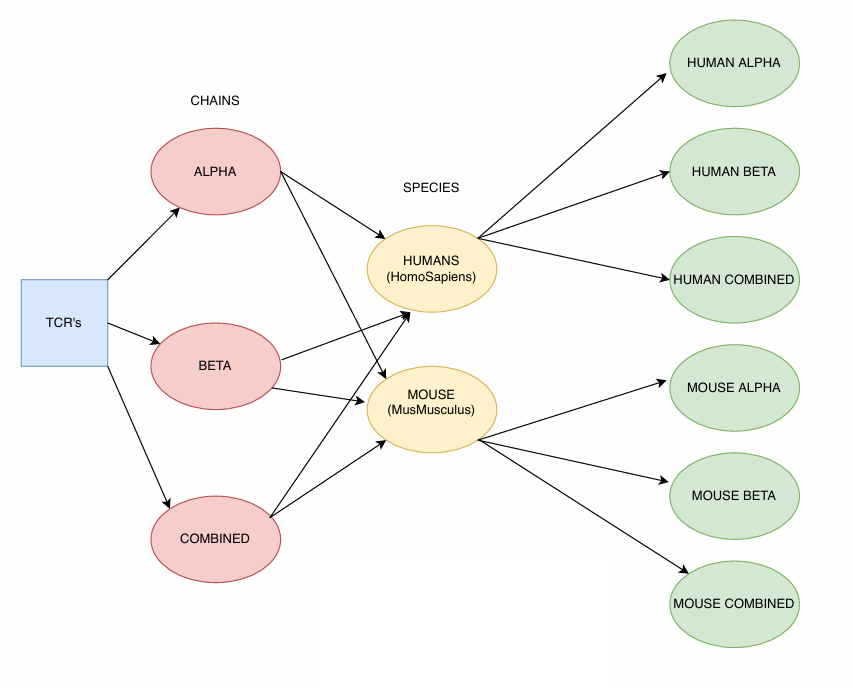
\includegraphics[height=5cm]{fig1.png}
		\caption{TCR Distance Matrix Calculation.}
		\label{fig}
	\end{figure}
	
	\subsubsection{GIANA} \
	
	GIANA\cite{b2} is a tool for analyzing immune cell receptor sequence data, which calculates the distance between sequences and similarity matrices. By passing the data of the alpha chain and the beta chain to the GIANA script separately, and specifying the output directory, the corresponding distance and similarity matrix files can be generated.
	
	\subsubsection{Levenshtein} \
	
	Levenshtein distance is a measure of how similar two strings are. Levenshtein distance is calculated by performing a series of insert, delete, and replace operations on one string to make it equal to another, and it represents the minimum number of edit operations required to convert one string to another.
	
	This article creates a function levenshtein\_distance\_matrix which is used to calculate the Levenshtein distance between a set of sequences. The function first calculates the length of the list of input sequences and creates an all-zero square matrix of size for the number of input sequences. Then, iterate over each pair of sequences in the sequence list, call the levenshtein\_distance function to calculate the edit distance between them, and fill in the result to the corresponding position of the all-zero square.
	
	\subsection{Classification}
	
	%\subsubsection{DecisionTreeClassifier} \
	
	%DecisionTreeClassifier is a tree-based supervised learning algorithm for classifying and regressing data. In the classification task, the decision tree generates a tree by performing a series of splits on the input features, with each split node representing a feature and each leaf node representing a category.
	%\begin{itemize}
	%	\item Feature Selection: Select the best split feature from the input features so that the split on that feature maximizes the purity of the data.
	%	\item Split nodes: Split the data based on the selected features to generate sub-nodes so that each sub-node contains samples that belong to the same category as much as possible.
	%	\item Recursive build: Repeat the above process for each child node until the stop condition is met.
	%	\item Prediction: The test sample is traversed along the branches of the tree to the leaf node, and the category of the leaf node is used as the prediction.
	%\end{itemize}
	
	%The split\_cdr3 function in this paper splits the TCR sequence and converts each amino acid in the sequence into a numeric code. 70\% of the data was used for training and 30\% for testing, the same random seed random\_state=42 was used for each experiment using the DecisionTreeClassifier model, the accuracy of each experiment was recorded, and the average accuracy of 20 experiments was calculated.
	
	
	\subsubsection{RnadomForestClassifier} \
	
	RandomForestClassifier is an ensemble learning method that consists of multiple decision trees, each trained on a different random subset, and ultimately averages their predictions. Compared with a single decision tree, random forests generally provide better generalization performance and are more robust to high-dimensional data and noise in the data.
	
	In this paper, the dataset is divided into a training set and a dataset, with 70\% of the data used for training and 30\% for testing, stratified sampling of the target variable (epitope) to keep the proportion of each category in the training set and test set up the same as in the original dataset, and RandomForestClassifier is used to build a model with 80 trees.
	
	\subsubsection{LogisticRegression} \
	
	This article uses the train\_test\_split function to allocate 20\% of the dataset to the test set and 80\% to the training set. Epitopes are the target variables, the labels of the antigen class to be predicted, which have been coded and set to random\_state=42 to ensure that the random results are the same every time you run the code.
	
	A logistic regression model was created, max\_iter=1000 was specified, the model was trained using the feature vector X\_train and the target variable y\_train of the training set, and the feature vector X\_test of the test set was predicted by using the trained model, and the prediction result was y\_pred, and finally the prediction accuracy was calculated.
	
	\subsubsection{SVM} \
	
	SVM (Support Vector Machine) is used for classification and regression analysis. The main idea is to find an optimal hyperplane to classify or regress the data. In the classification problem, the SVM tries to find an optimal decision boundary (i.e., hyperplane) that can separate data points of different classes, and maximize the distance from the boundary to the nearest data point (support vector).
	
	How SVM works: First, SVM maps data into a high-dimensional space where the data is linearly separable. Then, in this high-dimensional space, the SVM looks for an optimal hyperplane, that is, a decision boundary that can separate different classes of data points, so that the distance from the boundary to the nearest data point is maximized. For cases where it is non-linearly separable, SVM uses a kernel function to map the data to a higher-dimensional space, making the data linearly separable in this new space.
	
	\subsection{Clustering Methods}
	\subsubsection{Agglomerative Hierarchical Clustering} \
	
	Agglomerative Hierarchical Clustering\cite{b4} is a clustering algorithm that gradually merges data points into clusters, and represents the similarity relationship between data points through a tree-like structure. Agglomerative Hierarchical Clustering takes the distance between data points as a measure of similarity, and then gradually merges the data points into different clusters based on preset parameters (number of clusters, distance metric, and linking method).
	
	Mathematical Description:
	
	Start by treating each data point as a single cluster. Let $C = \{C_1, C_2, \ldots, C_N\}$ be the initial set of clusters where each $C_i$ contains a single data point. Define a similarity measure (or distance measure) $d(C_i, C_j)$ between two clusters $C_i$ and $C_j$.
	
	Find the closest (most similar) pair of clusters and merge them into a single cluster.Mathematically, if $C_i$ and $C_j$ are the closest pair, they are merged to form a new cluster $C_k$.
	
	After merging $C_i$ and $C_j$, update the distance matrix to reflect the distances of the new cluster $C_k$ to all existing clusters. 
	\begin{itemize}
		\item \textbf{Single Linkage}:
		
		$d(C_k, C_x) = \min(d(C_i, C_x), d(C_j, C_x))$
		\item \textbf{Complete Linkage}: 
		
		$d(C_k, C_x) = \max(d(C_i, C_x), d(C_j, C_x))$
		\item \textbf{Average Linkage}: 
		
		$d(C_k, C_x) = \frac{d(C_i, C_x) + d(C_j, C_x)}{2}$
		\item \textbf{Ward's Method}: Merge the pair of clusters that results in the minimum increase in total within-cluster variance after merging.
	\end{itemize}
	
	Repeat these steps until all data points are clustered into a single cluster of size $N$. As clusters are merged, a tree-like diagram called a dendrogram is created to record the sequences of merges. This dendrogram illustrates how each cluster is composed by branching out to its constituent elements.
	
	In this paper, the number of clusters was set to 5, and the similarity between the clustering results and the real labels and the clustering quality were evaluated by using the Adjusted Rand Index and Silhouette Score. The Adjusted Rand Index measures how similar the clustering results are to the real labels, with values between -1 and 1, with closer to 1 indicating that the clustering results are more similar to the real labels. The Silhouette Score measures the clustering closeness of each sample and ranges from -1 to 1, with closer to 1 indicating better clustering results.
	
	\subsubsection{DBSCAN} \
	
	DBSCAN is a popular clustering algorithm that identifies clusters of different shapes and sizes in a dataset, unlike methods such as K-means, DBSCAN does not require pre-specifying the number of clusters to be identified.
	
	For each point in the dataset, DBSCAN calculates how many points are within that eps (the maximum distance between two points, where one point is considered to be within the neighborhood of the other point, and the smaller the value, the more clustering) distance. If the count exceeds min\_samples (the minimum number of points required to form a dense area, higher values usually result in more points being treated as noise), then the point is marked as a core point; Starting from a core point, DBSCAN recursively finds all the points that are dense from that point and assigns them to the same cluster; Neither the core nor any core point where the direct density is reachable is marked as noise.
	
	In this paper, the DBSCAN algorithm is used to cluster the data in the distance matrix, and the eps parameter (neighborhood radius) and min\_samples parameter (minimum number of samples) are set, which determine the clustering results, which include the clustering label of each sample point and the label of the noise point. Finally, the contour coefficient of the clustering result is calculated using silhouette\_score. The contour coefficient is an index to measure the degree of tightness and separation of clustering results, and the value range is between [-1, 1], and the closer the value is to 1, the better the clustering result.
	
	In this algorithm, there are three values worthy of our attention, namely purity fraction, purity fraction and NMI\cite{b1}.
	\begin{itemize}
		\item Purity Fraction is defined as the percentage of pure clusters in the clustering output, where a pure cluster is one where all the TCRs are specific to the most common epitope in that cluster. 
		\item Purity Retention refers to the proportion of TCRs in all the pure clusters divided by the total number of TCRs in the test set. It provides an indication of how many TCRs in the dataset end up in pure clusters. 
		\item NMI is used to measure the mutual information between TCR clusters and epitope specificity, normalized by the sum of their individual entropies. It provides a standardized measure of the degree of association between the clustering of TCR sequences and their antigen specificities.
	\end{itemize}
	
	\subsection{Dimensionality Methods}
	\subsubsection{PCA} \
	
	PCA (Principal Component Analysis)\cite{b2}\cite{b3} is used to project a high-dimensional dataset into a low-dimensional space, by finding the principal variance directions (principal components) in the data, and then projecting the data onto these directions, so as to achieve dimensionality reduction of the data.
	
	Given a dataset \( X \) with \( n \) samples and \( d \) features, where \( X \) is an \( n \times d \) matrix, PCA aims to find a \( k \)-dimensional linear subspace that maximally preserves the variance of the original data. This subspace is defined by the \( k \) most important principal components.
	
	\text{Compute the mean vector of the data: } 
	$\bar{x} = \frac{1}{n} \sum_{i=1}^{n} x_i$
	
	Standardize the data: Subtract the mean vector from each sample to obtain the centered data: \( \tilde{X} = X - \bar{x} \)
	
	Compute the covariance matrix of the data: \( \Sigma = \frac{1}{n} \tilde{X}^T \tilde{X} \)
	
	Perform the eigendecomposition of the covariance matrix: $\Sigma = V \Lambda V^T$, where $V$ is the matrix containing the eigenvectors and $\Lambda$ is a diagonal matrix containing the eigenvalues.
	
	Select the top \(k\) eigenvectors corresponding to the largest eigenvalues: \(V_k = \begin{bmatrix} | & | & & | \\ v_1 & v_2 & \cdots & v_k \\ | & | & & | \end{bmatrix}\)
	
	Project the original data onto the selected principal components: \(Z = \tilde{X} V_k\)
	
	Through these steps, we obtain a lower-dimensional dataset \(Z\) with dimensions \(n \times k\). In this subspace, the variance of the data is maximally preserved, and the principal components \(v_i\) represent the most important directions in the data.
	
	\subsubsection{t-SNE} \
	
	t-SNE\cite{b2}\cite{b3} is a nonlinear dimensionality reduction algorithm designed to map high-dimensional data to two- or three-dimensional space. t-SNE first calculates the similarity between data points in the high-dimensional space, and then maintains this similarity relationship in the low-dimensional space, using the t-distribution to represent the distance between the data points in the low-dimensional space, which helps to preserve the local structure of the data.
	
	\subsubsection{UMAP} \
	
	UMAP\cite{b2}\cite{b3} (\emph{Uniform Manifold Approximation and Projection}) is a nonlinear dimensionality reduction algorithm, similar to t-SNE, but with faster computation speed and better ability to maintain the global structure than t-SNE.
	
	UMAP achieves dimensionality reduction and visualization through the following steps: first, calculate the similarity between data points, and then construct a neighborhood map to represent the local relationship between data points, second, optimize the manifold structure in the high-dimensional space to keep the distance of adjacent data points in the low-dimensional space as similar as possible, and finally, map the optimized manifold structure to the low-dimensional space to generate a new low-dimensional representation for visualization and analysis.
	
	In this paper, we create a UMAP instance, reducer, and use random\_state = 42 to ensure the reproducibility of the results, using the fit\_transform method to reduce the TCR distance matrix to a two-dimensional space.
	

	\subsection{Predict antigen specificity from sequence}
	%\subsubsection{Encoding} \
	
	This article first uses the fit\_transform method in the tool class LabelEncoder in scikit-learn to perform a test on 'gene', 'species', 'mhc.a', 'mhc.b', 'v.segm' and 'j.segm' encoding; the map method is used directly on 'mhc.class', 'MHCI' is mapped to 0, and 'MHCII' is mapped to 1.
	
	Next, the BLOSUM62 substitution matrix was loaded using the substitution\_matrices module in BioPython and a function encode\_sequence\_with\_blosum62 was defined to encode the sequence as a numerical representation of the BLOSUM62 matrix. Each amino acid in the sequence is traversed in a function using a for loop, and if the amino acid is present in the BLOSUM62 matrix, its encoding is added to the list of results, and if the amino acid is not in the BLOSUM62 matrix (such as gaps or special characters), it is represented by a zero vector of the same length as the number of rows in the matrix.
	
	Next, using a function GIANA\_encoder\_pd, the CDR3 sequence is encoded into a vector representation, first traversing each amino acid sequence, for each sequence, removing the C and J segments at the beginning, and the F segment at the end, encoding the sequence using a predefined M6 matrix.
	
	The 'epitope' column was encoded using LabelEncoder to convert categorical data into numeric labels. The LabelEncoder maps each different category to a unique number and assigns that number to the appropriate category.
	
	Use MinMaxScaler to normalize the data to ensure that individual features are within the same numerical range. For each feature, it is first reshaped into a single-column vector form, and then normalized to a range of 0 to 1 using the fit\_transform method.
	
	For each row, the encoded CDR3 sequence and the normalized eigenvalues are first concatenated, and then they are combined into a single array using the np.concatenate function. Finally, the resulting array contains the encoded CDR3 sequence and all the normalized eigenvalues, so that each row represents a complete sample eigenvector.
	
	
	\subsection{Figures and Tables}
	\paragraph{Positioning Figures and Tables} Place figures and tables at the top and 
	bottom of columns. Avoid placing them in the middle of columns. Large 
	figures and tables may span across both columns. Figure captions should be 
	below the figures; table heads should appear above the tables. Insert 
	figures and tables after they are cited in the text. Use the abbreviation 
	``Fig.~\ref{fig}'', even at the beginning of a sentence.
	
	\begin{table}[htbp]
		\caption{Table Type Styles}
		\begin{center}
			\begin{tabular}{|c|c|c|c|}
				\hline
				\textbf{Table}&\multicolumn{3}{|c|}{\textbf{Table Column Head}} \\
				\cline{2-4} 
				\textbf{Head} & \textbf{\textit{Table column subhead}}& \textbf{\textit{Subhead}}& \textbf{\textit{Subhead}} \\
				\hline
				copy& More table copy$^{\mathrm{a}}$& &  \\
				\hline
				\multicolumn{4}{l}{$^{\mathrm{a}}$Sample of a Table footnote.}
			\end{tabular}
			\label{tab1}
		\end{center}
	\end{table}
	
	\begin{figure}[htbp]
%		\centerline{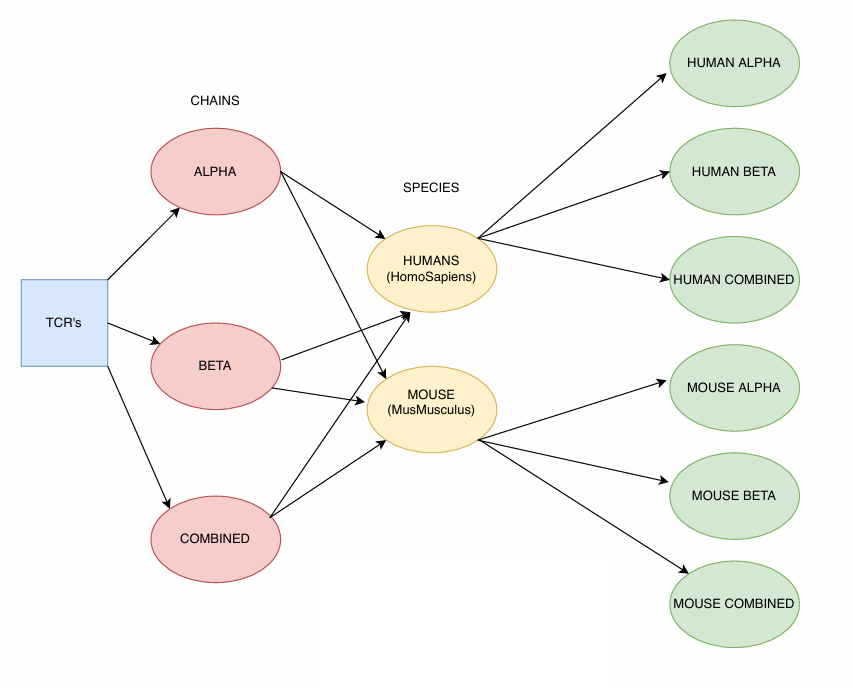
\includegraphics{fig1.png}}
		\caption{Example of a figure caption.}
		\label{fig}
	\end{figure}
	
	Figure Labels: Use 8 point Times New Roman for Figure labels. Use words 
	rather than symbols or abbreviations when writing Figure axis labels to 
	avoid confusing the reader. As an example, write the quantity 
	``Magnetization'', or ``Magnetization, M'', not just ``M''. If including 
	units in the label, present them within parentheses. Do not label axes only 
	with units. In the example, write ``Magnetization (A/m)'' or ``Magnetization 
	\{A[m(1)]\}'', not just ``A/m''. Do not label axes with a ratio of 
	quantities and units. For example, write ``Temperature (K)'', not 
	``Temperature/K''.
	
	
	\section{Data Description / Preparation}
	
	\subsection{Data Processing}
	\begin{itemize}
		\item Data filtering: Select specific columns ('complex.id', 'gene', 'cdr3', 'v.segm', 'j.segm', 'species', 'mhc.a', 'mhc.b', 'mhc.class', 'antigen.epitope') from the complete dataset to create a new DataFrame: filtered\_data.
		\item Missing value checking and processing: Because V and J are important factors when analyzing TCR characteristics, the rows with missing values in the columns 'v.segm' and 'j.segm' were removed from the new dataset filtered\_data.
		\item Data Segmentation and Reprocessing: In order to process the TCR sequences of alpha and beta chains separately, the data is divided into two new DataFrames based on the value of the 'gene' column: cdr3\_alpha\_df (rows containing 'gene' with 'TRA') and cdr3\_beta\_df (rows containing 'gene' with 'TRB') values. Remove the 'gene' column from the two new DataFrames, as the information in that column is already redundant after splitting the data.
		\item Data merging: cdr3\_alpha\_df and cdr3\_beta\_df were combined according to the columns 'complex.id', 'species', 'mhc.a', 'mhc.b', 'mhc.class', 'antigen.epitope'. Suffix different TCR strand feature columns, such as CDR3, V-segment, and J-segment, to distinguish datasets.
		
	\end{itemize}
	
	
	\section{Results and Discussion}
	{\color{blue}Reporting on the experiments with discussion on insights. Technical challenges are to be discussed here too.}
	
	\section{Further Work and Improvement}
	{\color{blue}Explore what can be done further based on the discussed insights and ways to improve.}
	
	\section{Conclusion}
	{\color{blue}A brief summary of the key insights in your report.}
	
	\begin{thebibliography}{00}
		%\bibitem{b1} H. Huang, C. Wang, F. Rubelt, et al., Analyzing the Mycobacterium tuberculosis immune response by T-cell receptor clustering with GLIPH2 and genome-wide antigen screening, Nature Biotechnology, vol. 38, no. 10, pp. 1194-1202, 2020.
		
		\bibitem{b1} H. Zhang, X. Zhan, and B. Li, "GIANA allows computationally-efficient TCR clustering and multi-disease repertoire classification by isometric transformation," Nature Communications, vol. 12, no. 1, pp. 4699, 2021.
		
		\bibitem{b2} M. Vujovic, K. F. Degn, F. I. Marin, et al., "T cell receptor sequence clustering and antigen specificity," \textit{Computational and Structural Biotechnology Journal}, vol. 18, pp. 2166-2173, 2020.
		
		\bibitem{b3} K. Mayer-Blackwell, S. Schattgen, L. Cohen-Lavi, et al., "TCR meta-clonotypes for biomarker discovery with tcrdist3 enabled identification of public, HLA-restricted clusters of SARS-CoV-2 TCRs," \textit{Elife}, vol. 10, p. e68605, 2021.
		
		\bibitem{b4} D. Müllner, "Modern hierarchical, agglomerative clustering algorithms,"
		\textit{arXiv preprint} arXiv:1109.2378, 2011.
		
	\end{thebibliography}
	
	\appendix
	{\color{blue}The document up to this section should be no more than 8 pages. The appendix section is optional. You can include additional material here, but it will not be marked.}
	
\end{document}
